\documentclass[letterpaper]{article}
\usepackage{natbib,alifeconf}

%\usepackage[pdftex]{graphicx}
\graphicspath{{./pdf/}}
\DeclareGraphicsExtensions{.pdf}

\usepackage{hyperref}

\title{Traders' Need for Harmony: Modelling Financial Markets Using
  the Golden Ratio} 

\author{Amaury Hernandez-Aguila and Mario Garcia-Valdez \\
\mbox{}\\
Tijuana Institute of Technology  \\
Division of Graduate Studies and Graduates \\
Tijuana, Mexico\\
\{amherag,mario\}@tectijuana.edu.mx}

\begin{document}
\maketitle

\begin{abstract}

\end{abstract}

\section{Introduction}
\label{introduction}

\citep{tirea2012stock}
\citep{chen2007fuzzy}
\citep{chakravarty2012pso}
\citep{pan2003joint}
\citep{osler2000support}
\citep{mantri2014artificial}
\citep{abdullah2012intervals}
\citep{kumar2014magic}
\citep{hellal2014wave}
\citep{zhen2010financial}
\citep{raberto2001agent}
\citep{seydel2006tools}
\citep{kotick1996introduction}
\citep{farmer2012complex}
\citep{otake2013can}
\citep{adebiyi2012stock}
\citep{chatterjee2002applications}
\citep{kotyrba2013methodology}
\citep{pan2005predicting}
\citep{kazem2013support}
\citep{livio2008golden}
\citep{murphy1999technical}
\citep{weckman2008integrated}
\citep{abounoori2014forecast}
\citep{prechter2001unconscious}
\citep{carney2005methodology}

\clearpage

\section{Related Work}
\label{related-work}

\clearpage

\section{Preliminaries}
\label{preliminaries}

Concept of pip. Concept of a trend, uptrend, downtrend. Resistance and
support. Retracement. Technical analysis. Fibonacci retracements and the
golden ratio. Timeframe. Open, high, low, close prices.

\clearpage

\section{Proposed Method}
\label{proposed-method}

Following the hypothesis stated in Section \ref{introduction},
individuals who are trading in a financial market should constantly % trading in a financial market?
``feel'' that the appropriate amount of units a trend will retrace
should follow certain natural pattern, which should be close to the
golden ratio, with respect to this trend. 
%Maybe they dont know is a golden ratio,  so maybe 
%...should follow certain natural pattern %% Lo que es el golden ratio
%se va a explicar en Preliminaries
If this hypothesis
is true, many upwards or downwards movement in a financial market %every -->> many
should be the cause for a retracement that follows a golden
proportion with respect to this upwards or downwards movement. One can
then consider these possible retracements as support or resistance
levels, because after the retracement occurs, traders should stop
trading the market in that direction and change their position from
buying to selling, and vice versa. If all of these support and
resistance levels are calculated, one can see, at the current or at
any given price, if there is more resistance for the market to follow an
uptrend or a downtrend. These are the concepts behind the proposed
method, and it will be explained further in the following paragraphs,
and how they can be used to create a model of a financial market.

In technical analysis, traders need to identify a previous trend to 
% 
% Explain a little more, why? In order to find support o resistence levels
% a technique that is often used in technical analysis, is ... 
% because ... %%% El método de retrasos de Fibonacci lo voy a explicar
% en Preliminaries
draw Fibonacci retracements according to this previous
movement. This process is subjective, and entirely depends on the
opinion of the trader, as there is not a method to reliably determine
where exactly a trend starts and ends. For the proposed method, this
problem is alleviated by considering every continuous upwards or
downwards movement in close prices for a given timeframe to be a
trend, therefore eliminating the need for an opinion to determine a
high and a low to draw the Fibonacci retracements. %% Why is alliviated 

After calculating all the uptrends and downtrends, retracement levels
are calculated for every of these movements. The proportions that are taken
into consideration to calculate the retracements are: 23.6\%, 38.2\%,
50\%, 61.8\%, 76.4\%, and 161.8\%, as these are the most widely used
\ref{murphy1999technical}. For example, considering the 1-hour
timeframe, if the EUR vs USD exchange market moved (in close prices)
from 1.1000 to 1.1050 in the first hour, then from 1.1050 to 1.1100 in
the second hour, and finally from 1.1100 back to 1.1050 in the third
hour, following the procedure mentioned before, one would only take
into consideration the first two hours as an uptrend, and the third
hour as a downtrend. In the uptrend, a movement of 100 pips occured,
while in the downtrend the market fell 50 pips. As a consequence of the
uptrend, the following seven resistance levels are generated: 1.1076,
1.1062, 1.1050, 1.1038, 1.1024, 1.1000, and 1.0938. As a consequence
of the downtrend, the following seven resistance levels are generated:
1.1062, 1.1069, 1.1075, 1.1081, 1.1088, 1.1100, and 11131.
%%
%% Can we explain this with a Figure? %% Qué cosa exactamente? Alguna
%% idea de qué poner?

The process described before will generate a list of prices that
represent resistance levels, prices where traders are most likely to
stop trading in their current direction, and revert to the opposite
direction. This list of prices needs to be reduced by counting the
number of instances each price is mentioned, giving as a result a list
of prices with their strengths or importances as resistance
levels. Finally, as an additional step for this stage of the process,
the price levels are weighted according to their time of occurrence,
i.e., resistance levels generated by earlier prices are weighted more
than those occurred later in the time series.
%%
%% Explain first the goal of the method, something like:
%% The goal of this process is to give a weight to each price
%% indicating the strength to support or resist according to
%% the perceived adherence to the golden rule? %% Dónde lo pongo, al
%% principio del párrafo de arriba?

The final generated list of resistance levels can then be used to
forecast the following close prices. For example, if there are
stronger resistance levels above the current price than below it, most
traders will favor to follow a downward movement. Before doing this,
one must determine how many price levels above and below the current
price are going to be considered to make a decision. This parameter
can be established in an arbitrarily manner, or by using an
optimization method such as hill climbing, simulated annealing, or a
genetic algorithm.

By examining the results of applying this method as is defined in the
previous paragraphs (in Section \ref{results}, Figures
\ref{eurusd60-r}, \ref{gbpusd60-r}, \ref{audusd60-r}, %change?
\ref{usdcad60-r}, and \ref{usdchf60-r}), one can notice that after
5000 hours of trading, some currency exchange markets generated
profits. Nevertheless, what is interesting is not the profit generated
by the method, but the consistency at which the profits increase or
decrease. As a result of this observation, one can deduce that the
method of taking a decision based on the strength of the resistance
levels above or below a price level sometimes flips: these resistance
levels sometimes act as a repulsion force, and sometimes as an
attraction force. Taking this into consideration, one can implement
the previously discussed method in such a way that, when the market is
no longer obeying the resistance levels as a repulsion force, the
method can start considering them as an attraction force, and vice
versa. The experiments presented in Section \ref{experiments}
implement all of the steps described in this Section.

\clearpage 

\section{Experiments}
\label{experiments}

The method described in Section \ref{proposed-method} was implemented
and tested with the following currency exchange markets: EUR vs USD,
GBP vs USD, AUD vs USD, USD vs CAD, and USD vs CHF, all of them in a
1-hour timeframe. The size of these datasets consisted on 5000 hours,
starting from the 27th of January, 2015, at 21:00, to the 22nd
of January, 2016, at 12:00. The time zone for these dates is +1 GMT.

\clearpage

\section{Results}
\label{results}

EUR vs USD

\begin{figure}[!t]
  \centering
  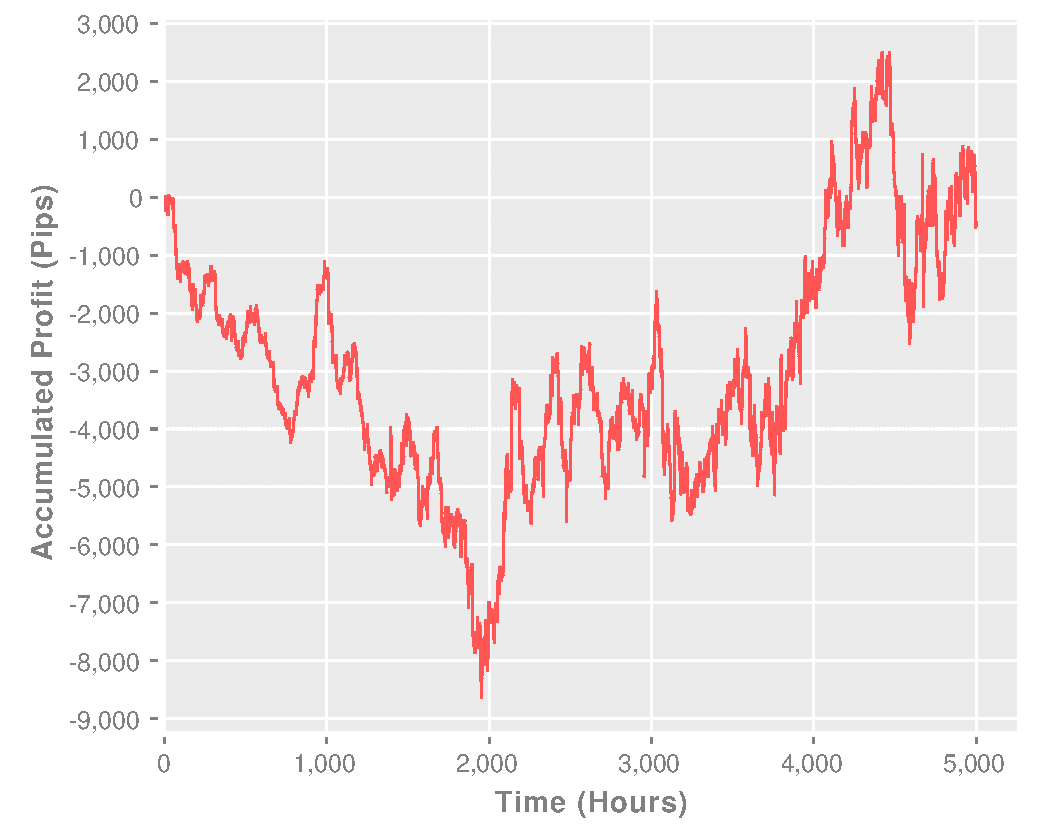
\includegraphics[width=3.0in]{eurusd60-r}
  \caption{EUR vs USD, 1 Hour Sessions, Raw}
  \label{eurusd60-r}
\end{figure}

\begin{figure}[!t]
  \centering
  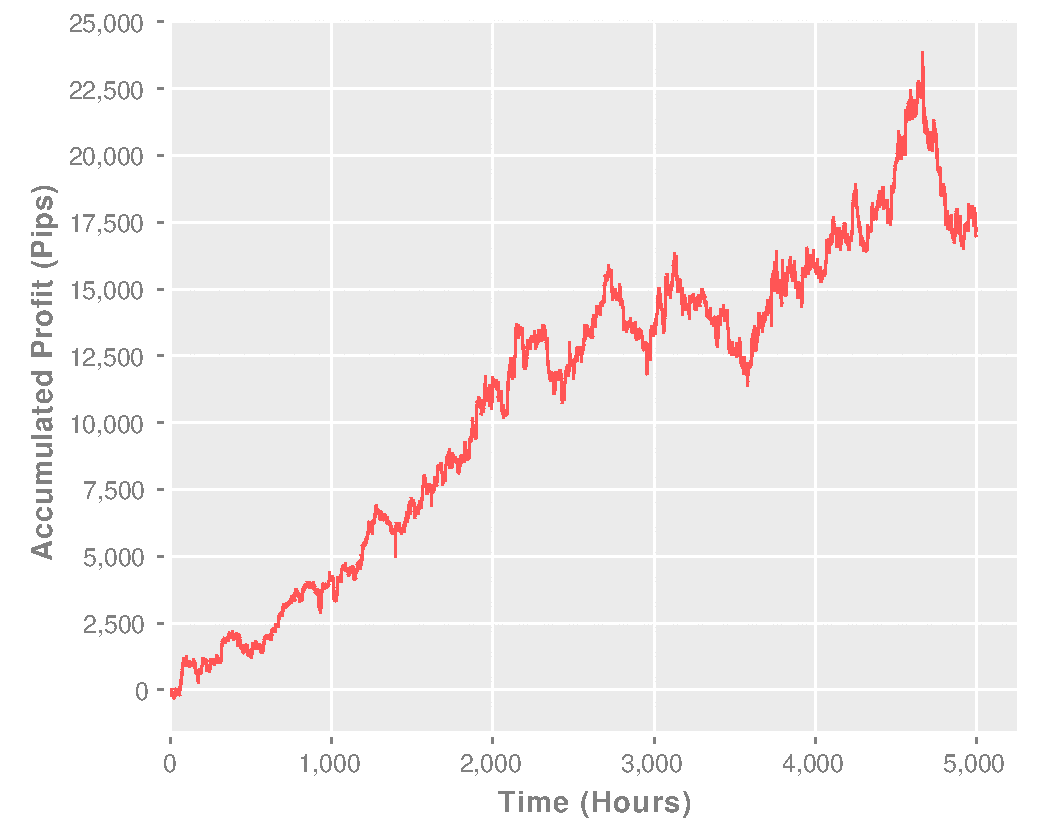
\includegraphics[width=3.0in]{eurusd60-of}
  \caption{EUR vs USD, 1 Hour Sessions, Full}
  \label{eurusd60-of}
\end{figure}

\begin{figure}[!t]
  \centering
  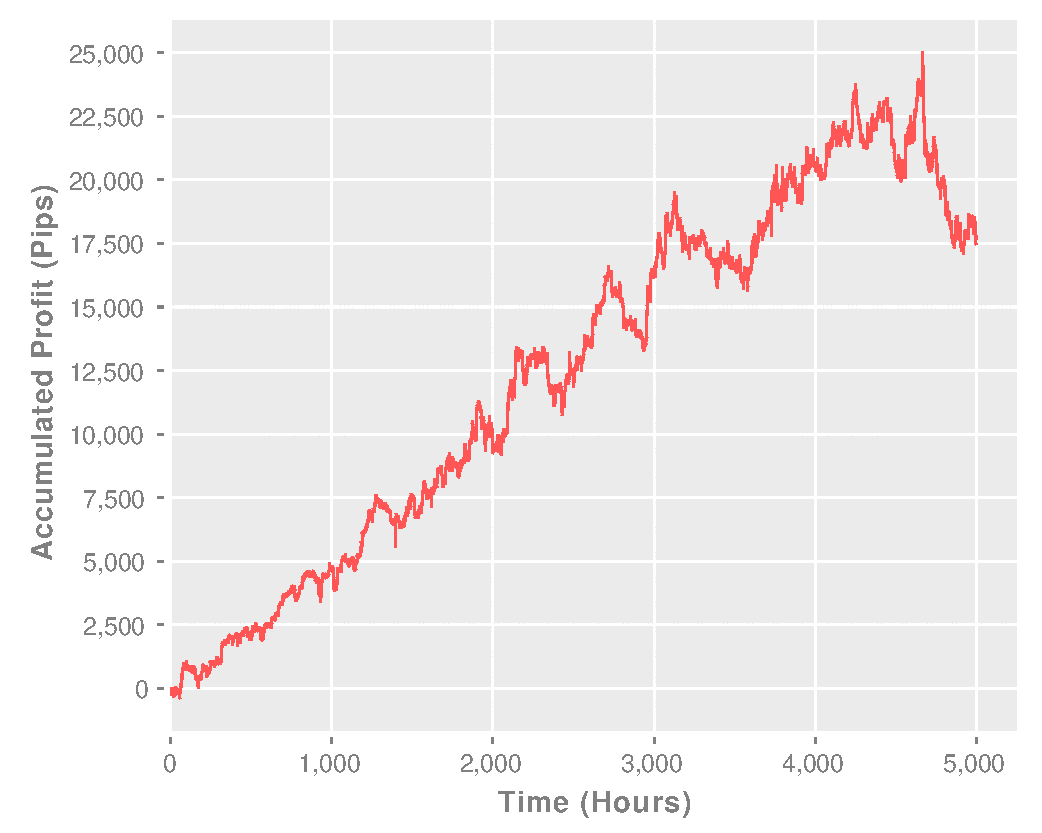
\includegraphics[width=3.0in]{eurusd60-op}
  \caption{EUR vs USD, 1 Hour Sessions, Partial}
  \label{eurusd60-op}
\end{figure}

GBP vs USD

\begin{figure}[!t]
  \centering
  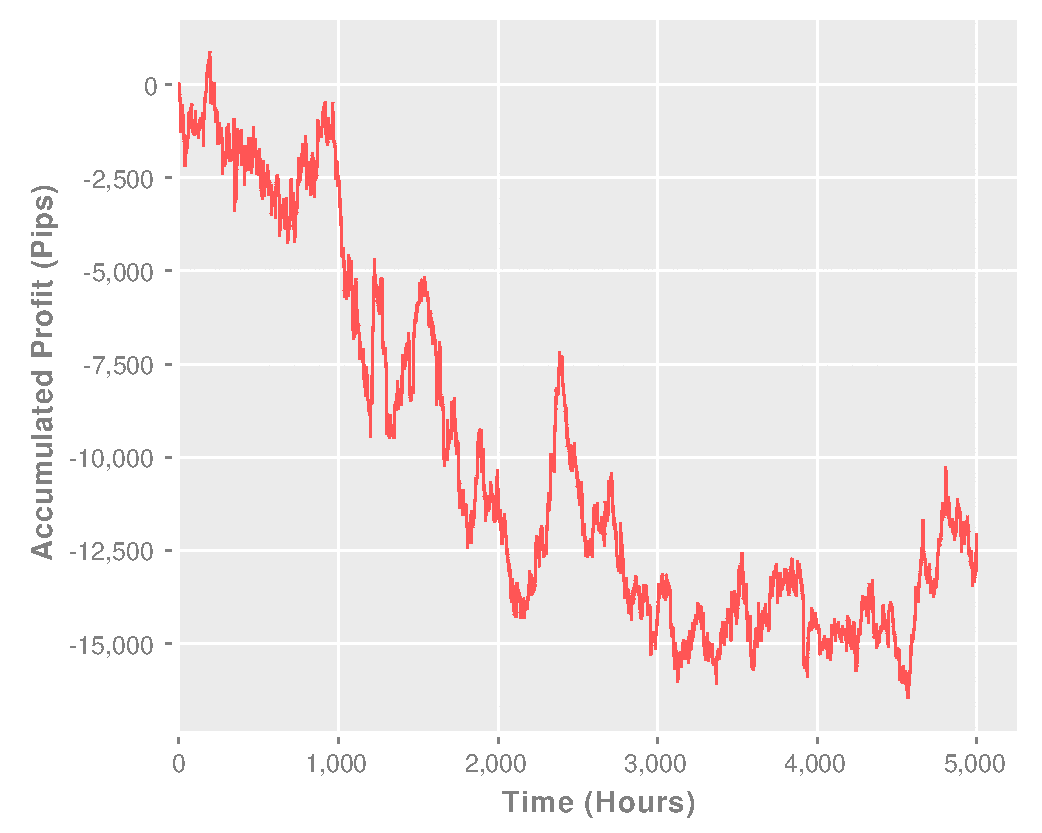
\includegraphics[width=3.0in]{gbpusd60-r}
  \caption{GBP vs USD, 1 Hour Sessions, Raw}
  \label{gbpusd60-r}
\end{figure}

\begin{figure}[!t]
  \centering
  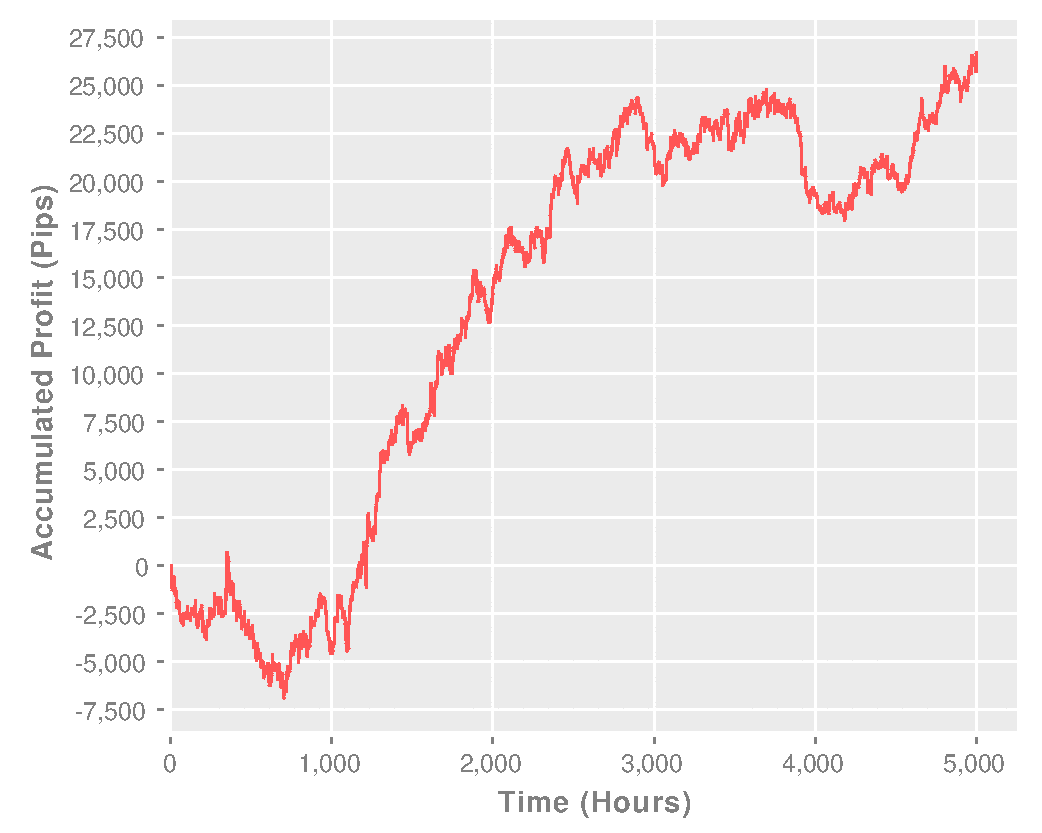
\includegraphics[width=3.0in]{gbpusd60-of}
  \caption{GBP vs USD, 1 Hour Sessions, Full}
  \label{gbpusd60-of}
\end{figure}

\begin{figure}[!t]
  \centering
  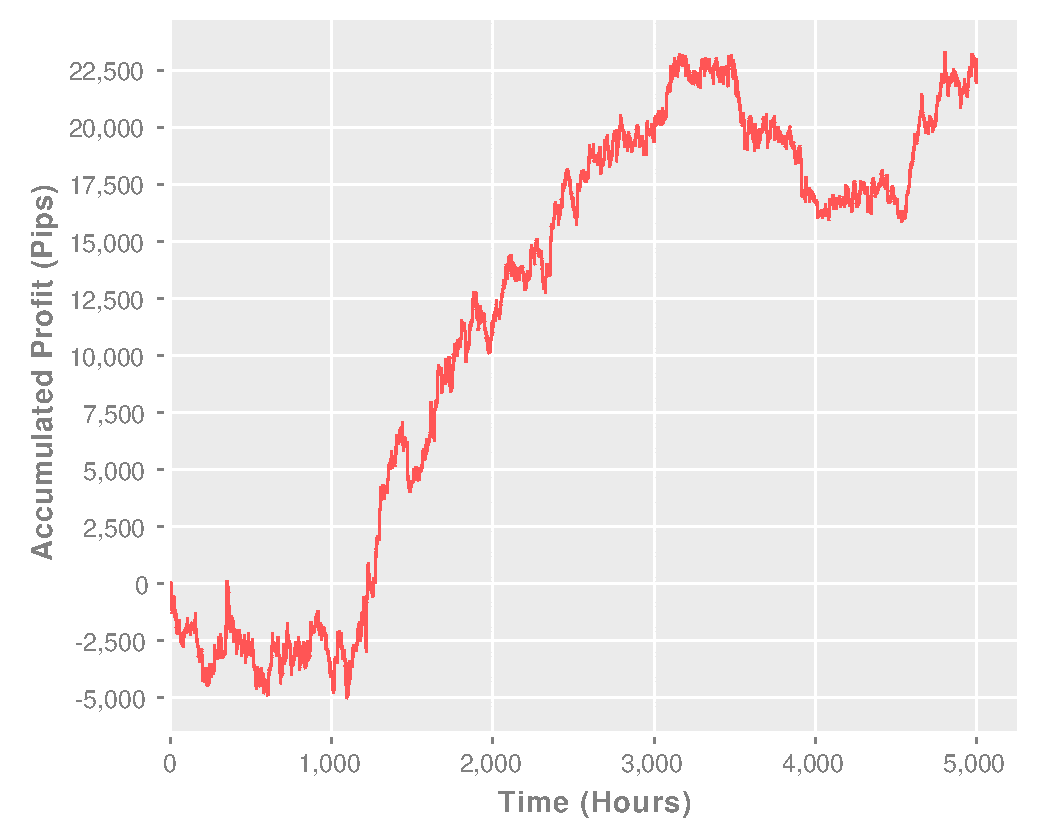
\includegraphics[width=3.0in]{gbpusd60-op}
  \caption{GBP vs USD, 1 Hour Sessions, Partial}
  \label{gbpusd60-op}
\end{figure}

AUD vs USD

\begin{figure}[!t]
  \centering
  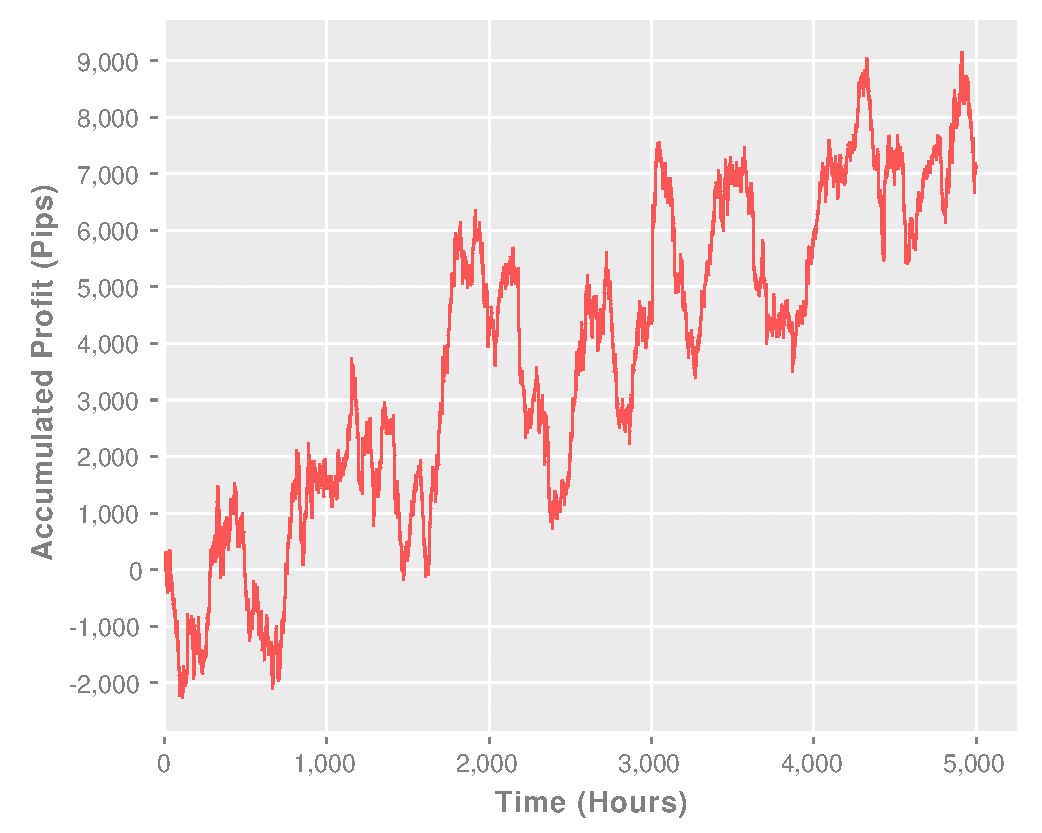
\includegraphics[width=3.0in]{audusd60-r}
  \caption{AUD vs USD, 1 Hour Sessions, Raw}
  \label{audusd60-r}
\end{figure}

\begin{figure}[!t]
  \centering
  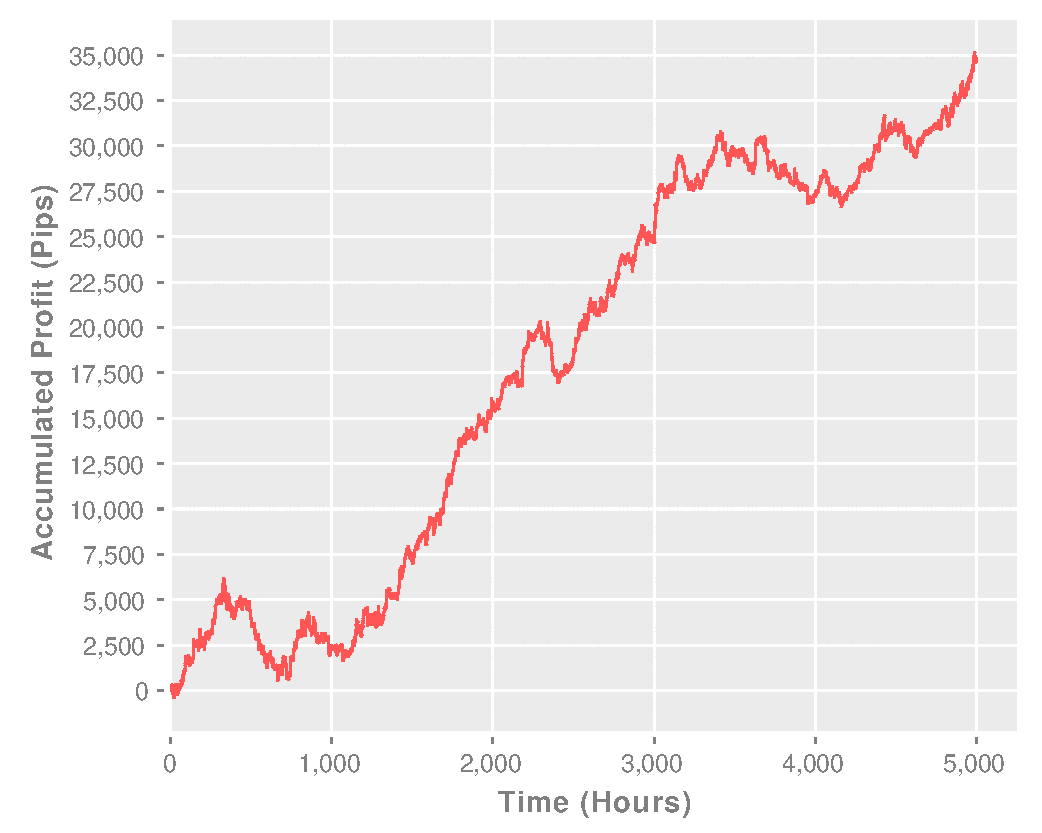
\includegraphics[width=3.0in]{audusd60-of}
  \caption{AUD vs USD, 1 Hour Sessions, Full}
  \label{audusd60-of}
\end{figure}

\begin{figure}[!t]
  \centering
  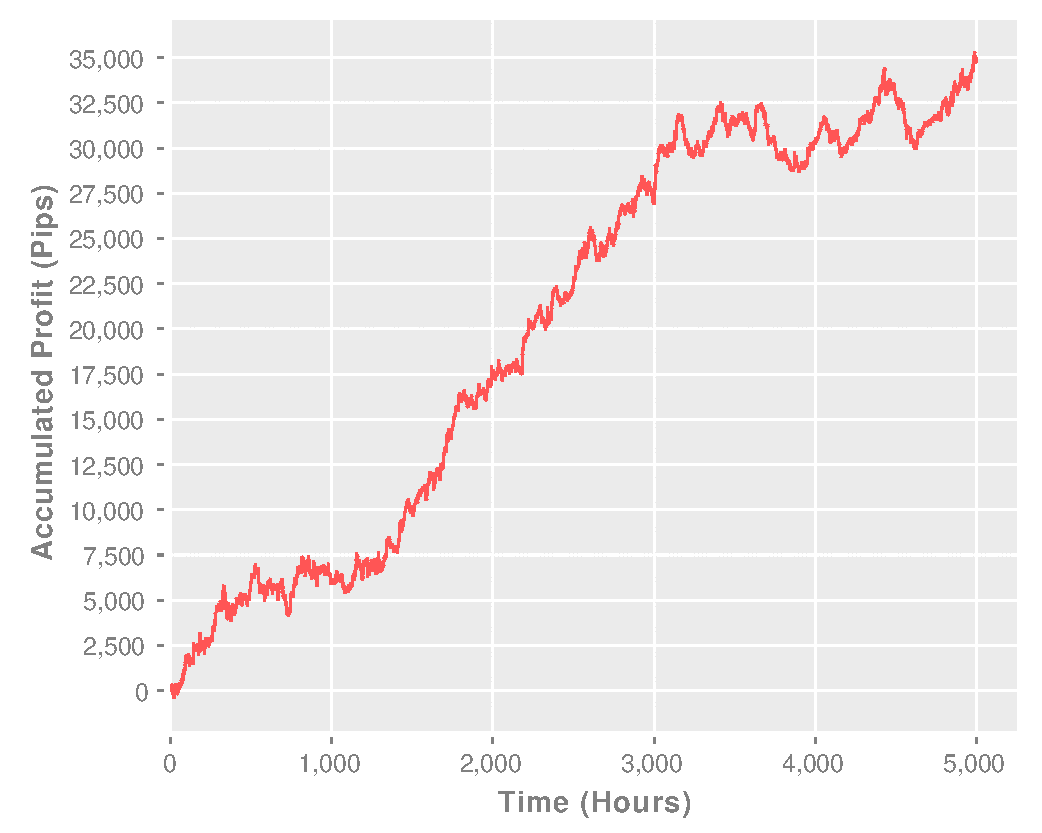
\includegraphics[width=3.0in]{audusd60-op}
  \caption{AUD vs USD, 1 Hour Sessions, Partial}
  \label{audusd60-op}
\end{figure}

USD vs CAD

\begin{figure}[!t]
  \centering
  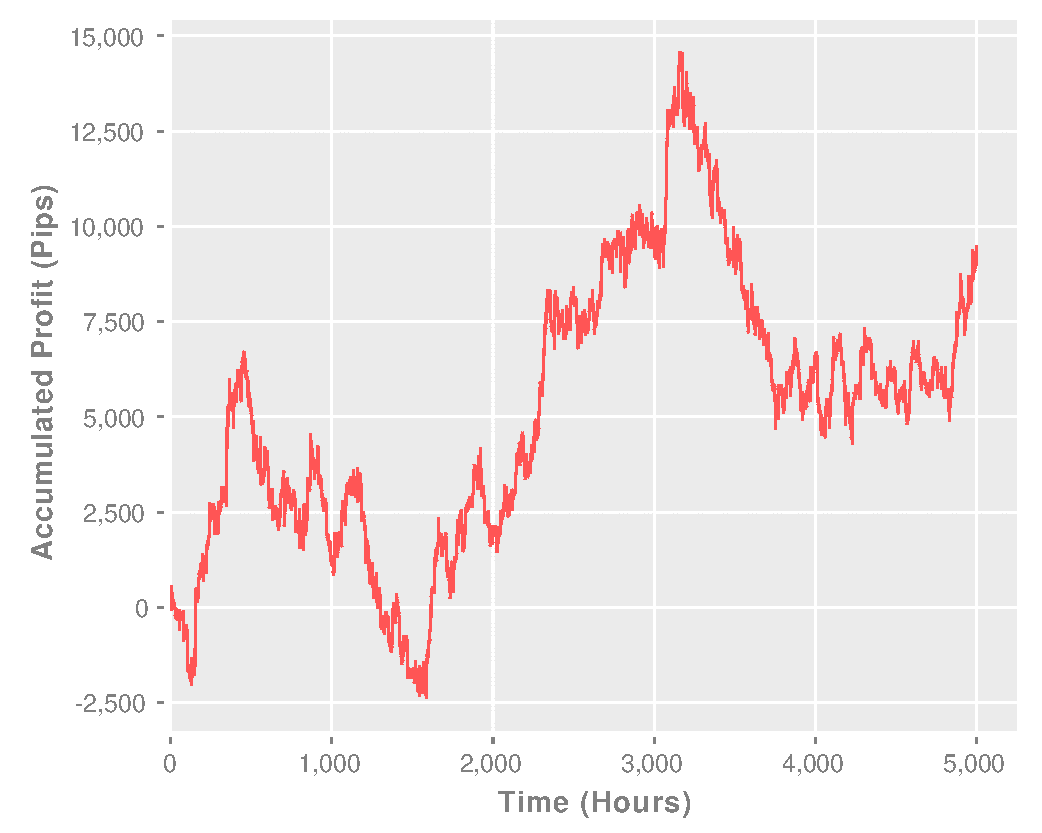
\includegraphics[width=3.0in]{usdcad60-r}
  \caption{USD vs CAD, 1 Hour Sessions, Raw}
  \label{usdcad60-r}
\end{figure}

\begin{figure}[!t]
  \centering
  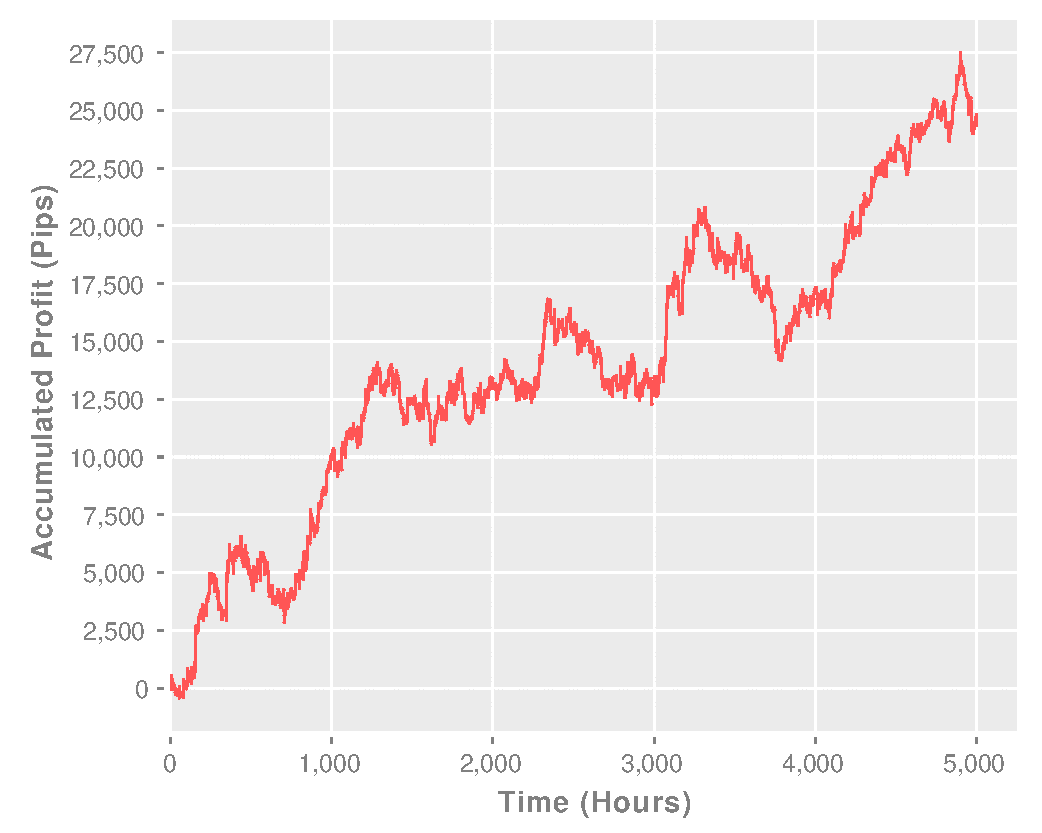
\includegraphics[width=3.0in]{usdcad60-of}
  \caption{USD vs CAD, 1 Hour Sessions, Full}
  \label{usdcad60-of}
\end{figure}

\begin{figure}[!t]
  \centering
  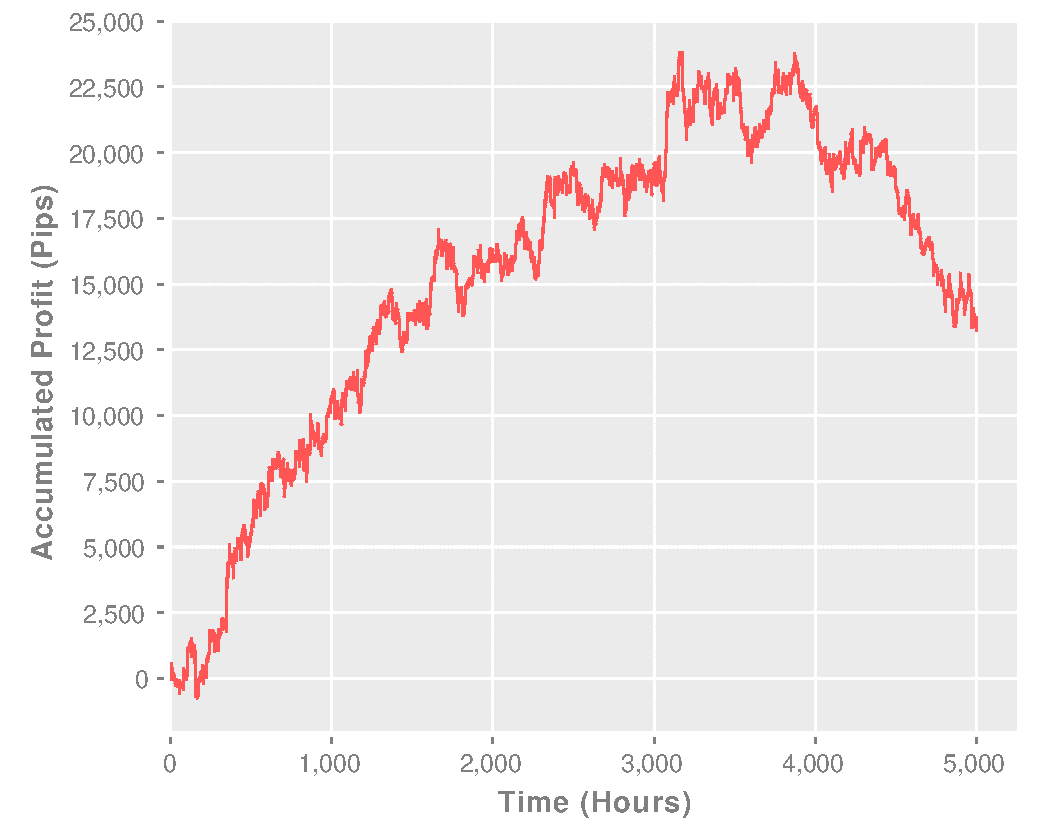
\includegraphics[width=3.0in]{usdcad60-op}
  \caption{USD vs CAD, 1 Hour Sessions, Partial}
  \label{usdcad60-op}
\end{figure}

USD vs CHF

\begin{figure}[!t]
  \centering
  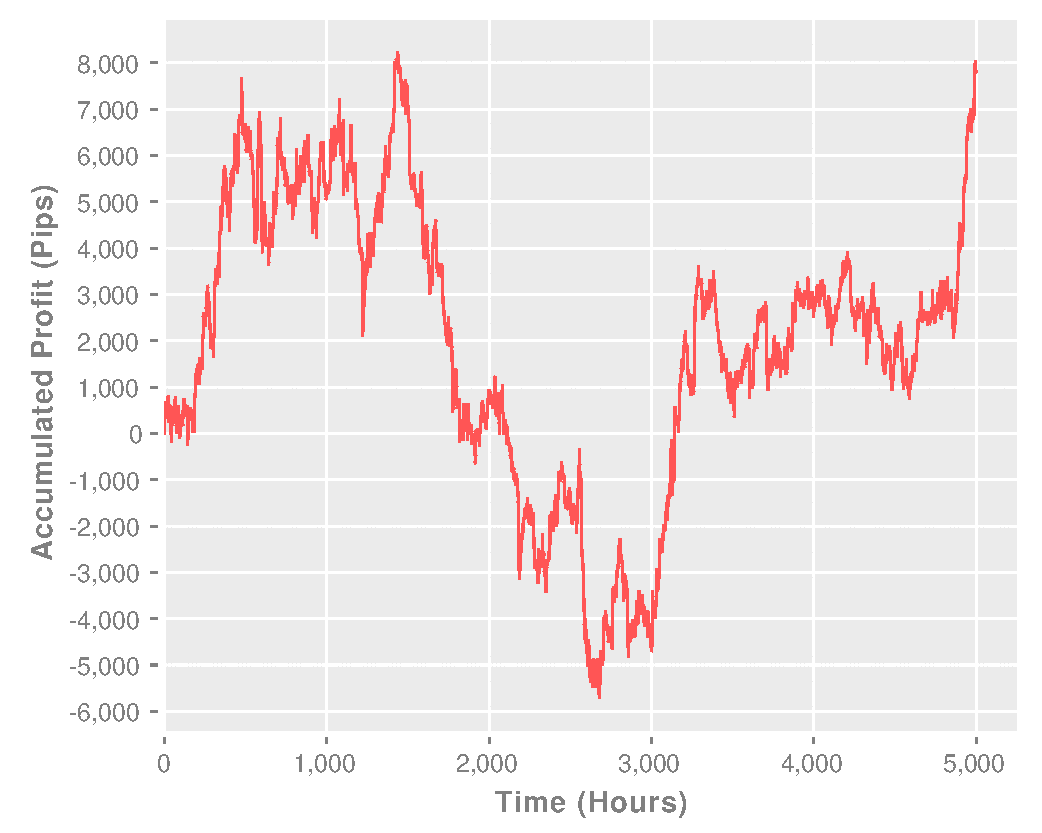
\includegraphics[width=3.0in]{usdchf60-r}
  \caption{USD vs CHF, 1 Hour Sessions, Raw}
  \label{usdchf60-r}
\end{figure}

\begin{figure}[!t]
  \centering
  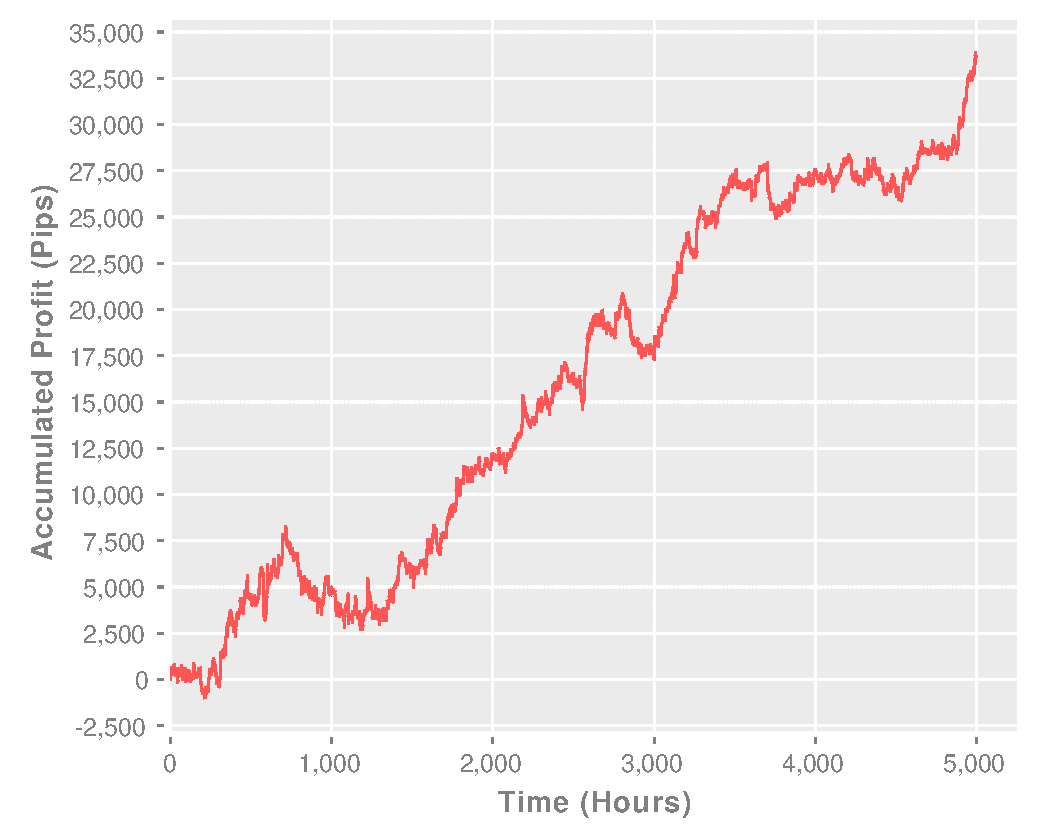
\includegraphics[width=3.0in]{usdchf60-of}
  \caption{USD vs CHF, 1 Hour Sessions, Full}
  \label{usdchf60-of}
\end{figure}

\begin{figure}[!t]
  \centering
  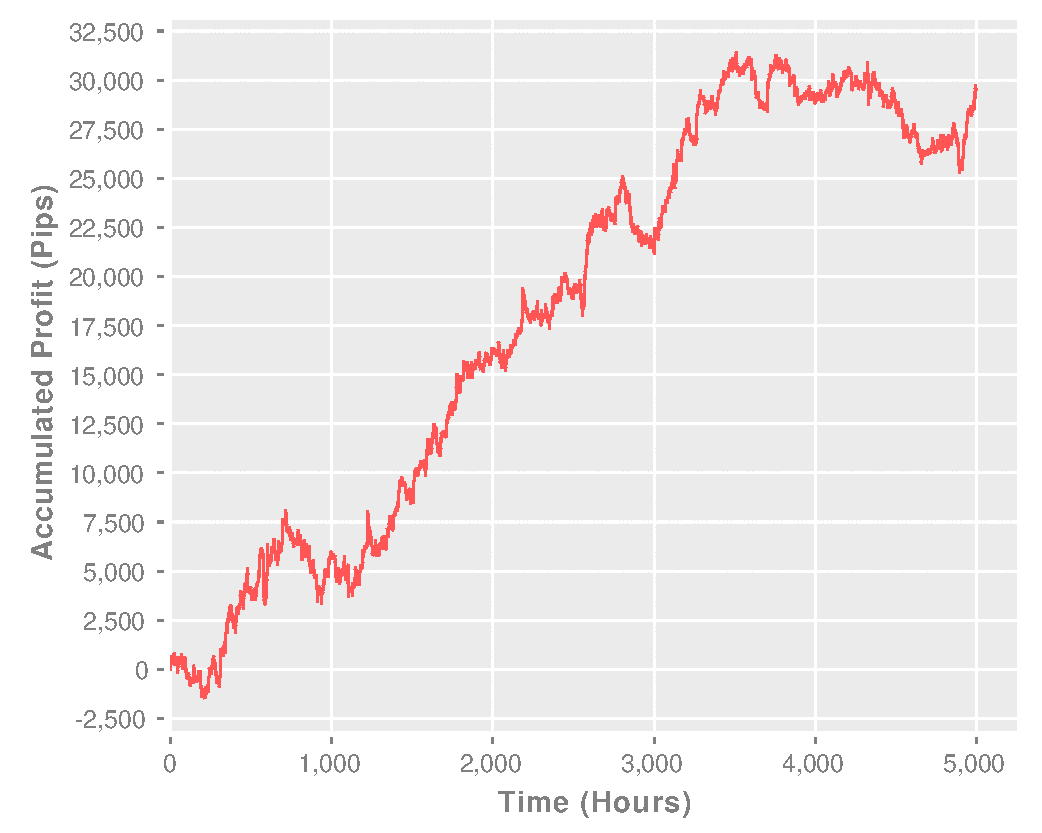
\includegraphics[width=3.0in]{usdchf60-op}
  \caption{USD vs CHF, 1 Hour Sessions, Partial}
  \label{usdchf60-op}
\end{figure}

\clearpage

\section{Conclusion}
\label{conclusion}
\section{Future Work}
\label{future-work}

\clearpage

\bibliographystyle{apalike}
\bibliography{paper}

\end{document}
